\chapter{Related Work}
\label{chp:relwork}

\section{BitTorrent}
\bt~\cite{2003:bittorrent:cohen} is a file distributed system on top of peer-to-peer network. Static \texttt{.torrent} file, which contains information such as tracker addresses and unique hash value of this swarm, is created by peer who wants to publish their files. \textit{Tracker} is responsible for monitors the distribution and progress of file and peers in a swarm. Peer uses information in \texttt{.torrent} file to connect each other.

% tit-for-tat, choking, unchoke, optimistic unchoke
\todo{cite cheating peers/freeloader/hit-n-run behavior}
\todo{cite choke/unchoke algorithm}
In \bt, it is desirable to have many peers upload piece of file to the swarm. This way, swarm can be \textit{healthier}, and overall download speed can increase. However, many peers become a \textit{leecher}, which quit the swarm when his download finished. \bt~uses \textit{tit-for-tat} mechanism to reward good behavior and punish bad behavior. To force cooperation of other peers, \bt~ implement \textit{choking algorithm}. Choking algorithm is an algorithm to temporarily refuse uploading piece of file to a particular peer. Usually, an uploader has a limited number of unchoked slots. By observing other peers, choking algorithm decides which peer a particular piece will be sent or not sent to. If we unchoke a peer, it means we consider to upload a piece to that peer. For starters, it is usually useful to execute \textit{optimistic unchoking}. Optimistic unchoking is an algorithm to unchoke a peer regardless of its activity in a swarm. This gives a peer a chance to increase his upload rate by providing more content.

% peer discovery DHT, PEX, LSD
\subsection{Peer Discovery}
One of the integral part in \bt~protocol is peer discovery. With numerous known peers, the algorithm will have more option on which peer to unchoke. State of the swarm itself often represented by the peer belong to that swarm. In \bt, there are four methods to discover new or update peer. 

\subsubsection{Tracker Peer Announce}
In original design of \bt, it uses tracker to allow peer discover each other \cite{2003:bittorrent:cohen}. Tracker tends to use random and limited list of peers. Peer contact tracker periodically to expand their peer dictionary. This act of requesting peer to tracker is called \textit{announce}.	Usually, most tracker has a policy about recommended interval when to recontact for getting new peers. Violate this policy can result a particular peer blocked.

\subsubsection{Distributed Hash Table (DHT)}
\todo{DHT performance?}
Originally, peer needs to contact tracker to fetch new peer address and file information. This makes \bt~very dependent on centralized system which vulnerable to single point of failure. In 2008, Distributed Hash Table (DHT) was proposed \cite{2008:dht:loewenstern}. Towards a ``trackerless'' \bt~system, DHT allows each peer to become a tracker. DHT stores peer contact information with defined key-space as ``node ID''. Each peer stored other peer's node ID and its address in their own routing table. A ``distance'' is measured on two node ID to define how close those two. ``Distance'' also can be measured between infohash of a torrent and node ID.

To enrich its peer dictionary, a node can compare a torrent's infohash and node ID in its routing table. If the distance under the threshold, it contacts that node to ask the information of the swarm, which includes the peer list. If contacted node do not know this torrent, it will respond with another node in its table which closest to the provided infohash.

\subsubsection{Peer Exchange (PEX)}
To increase the chance of getting higher downloading speed, having up to date peer is desired. This can be achieved by contacting tracker or using DHT. Reducing the interval of contacting tracker can result in getting a number of updated peer sooner, however, it will put a burden on the tracker itself. Peer Exchange (PEX )\cite{2015:PEX:the8472} is proposed to tackle this problem. PEX used list of peers that bootstrapped from another mechanism. This mechanism allows contacting known peer directly to get and give up-to-date information on swarm. Theoretically, it can keep this swarm together if trackers are down. Specification mentioned in \cite{2015:PEX:the8472} stated a restriction such as number of request per minute and number of peer added or removed in a PEX message.

\subsubsection{Local Service Directory (LSD)}
To increase the performance when downloading from a swarm, it is preferable to get the file from local network if available. Local service directory (LSD) permit this by discover peers that are in the same local network. The transfer rate is much higher compared to other type of peers. In short, LSD uses multicast-like mechanism which broadcast infohash of a torrent.

\section{Tribler}
Tribler\footnote{\url{https://www.tribler.org/}} is peer-to-peer file sharing application that compatible with \bt~protocol \cite{2008:tribler:pouwelse}. Tribler focused on security, fully decentralized system, and anonymity. Starts with ABC (Another \bt~Client), Tribler currently provides content discovery, channels concept, and reputation management in fully distributed manner.

Tribler is well known for its anonymity and secure interface on top of \bt~ network. In 2014, Tribler published a specification on its anonymity feature\footnote{\url{https://github.com/Tribler/tribler/wiki/Anonymous-Downloading-and-Streaming-specifications}}. It uses Tor-like onion routing with purely distributed mechanism. A year later, \citeauthor{2015:tunnel:ruigrok} on his work completed the \texttt{tunnel community} which emphasize end-to-end encryption in Tribler. This comes with several drawbacks. First is performance degradation. Adding layers of privacy comes with increasing the amount of cryptography operation which slows down end-to-end downloading activity \cite{2015:tunnel:ruigrok}.

All of the Tribler main components such as end-to-end encryption, channel discovery, and many others relied in database and dissemination system called \texttt{Dispersy} \cite{2013:dispersy:zeilemaker}. Dispersy maintain and perform the communication between Tribler peers in fully decentralized manner. Dispersy able to circulate the message in one-to-one or one-to-many within a group of node called \texttt{community}. User can adapt and implement its desired \textit{community} by itself. It is including how, what, and where the communication will occur.

Tribler implements several Dispersy \textit{communities} on its core function. \citeauthor{2016:tribler-techdebt:vos} summarize the recent community in Tribler. As shown in table \ref{tbl:community}, important features such as channel discovery, search within community, end-to-end Tor-like operations, and currency mechanism. \textit{Channel} is a collection of torrent that has extra capabilities such as vote system, spam prevention, and comment (social) attributes. Every user can create his own channel, add and remove torrent to it, and maintain its activity.

\begin{table}[tbp]
	\centering
	\caption{Overview of implemented Dispersy community in Tribler \cite{2016:tribler-techdebt:vos}.}
	\label{tbl:community}
	\begin{tabular}{|l|p{11cm}|}
		\hline
		\rowcolor[HTML]{EFEFEF} 
		\multicolumn{1}{|c|}{\cellcolor[HTML]{EFEFEF}{\color[HTML]{333333} \textbf{Community Name}}} & \multicolumn{1}{c|}{\cellcolor[HTML]{EFEFEF}{\color[HTML]{333333} \textbf{Purpose}}}                                                                                                                                     \\ \hline
		\textit{AllChannel}                                                                          & Used to discover new channels and to perform remote channel search operations.                                                                                                                                           \\ \hline
		\textit{BarterCast4}                                                                         & While currently disabled, this community was used to spread statistics about the upload and download rates of peers inside the network and has originally been created as a mechanism to prevent free-riding in Tribler. \\ \hline
		\textit{Channel}                                                                             & This community represents a single channel and is responsible for managing torrents and playlists inside that channel.                                                                                                   \\ \hline
		\textit{Multichain}                                                                          & This community utilizes the blockchain technology and can be regarded as the accounting mechanism that keeps track of shared and used bandwidth.                                                                         \\ \hline
		\textit{Search}                                                                              & This community contains functionalities to perform remote keyword searches for torrents and torrent collecting operations.                                                                                               \\ \hline
		\textit{(Hidden)Tunnel}                                                                      & This community contains the implementation of the Tor-like protocol that enables anonymity when downloading content and contains the foundations of the hidden seeder services protocol, used for anonymous seeding.     \\ \hline
	\end{tabular}
\end{table}

\subsection{Libtorrent}
Another Tribler dependency is \textit{libtorrent}\footnote{\url{http://libtorrent.org/}}. With \bt~is just a collection of specification, it free to be implemented with any languages. One of the implementation in \texttt{C++} is \textit{libtorrent}. \textit{libtorrent} also has \texttt{python} binding which the same language as Tribler implementation. \textit{Libtorrent} started in 2003 by Arvid Norberg. \textit{Libtorrent} is used by many torrent client such as Deluge, qBittorrent, Free download managers, and many others.

\subsubsection{Share Mode}
One of the crucial feature used in this work is \textit{share mode} \footnote{Core code of share mode can be found in \url{https://github.com/arvidn/libtorrent/blob/master/src/torrent.cpp\#L9586-L9727}}. Initial work performed by \citeauthor{2015:creditmining:capota} also used this feature\cite{2015:creditmining:capota}. By enabling share mode, it means that one is not interested in downloading the file, but gaining higher share ratio. It is done by download as little as possible and upload as much as possible. Share mode only download a torrent where it has sufficient capacity. A torrent downloaded in share mode may never finish as \textit{libtorrent} only download piece of a torrent which satisfied the share mode requirements. Share mode can be enabled per torrent basis.

Share mode algorithm works heuristically as it estimates the rarest piece available in the swarm based on participated peers. First, it tries to find whether there is a piece which nobody has (line \ref{alg:l_lts:missingp}). Note that in line \ref{alg:l_lts:disconnectpeers}, libtorrent disconnect some of the seeder because we need to connect to the leecher later. This case is considered if there are too many seeder in our connection pool. Next, the number of missing pieces is decreased linearly with the number of seeder. This is based on assumption that both of us and other seeder can upload at least one piece each (line \ref{alg:l_lts:reducemissing}). To keep the performance, downloading piece activity is stacked until more than 5\% of the number to be downloaded (line \ref{alg:l_lts:retdling}). To determine rarest piece, libtorrent count the number of peer that has that piece. The number of peer on the rarest piece is termed \textit{rarity}. Share mode ensure that we only download the rarest piece available in the network (line \ref{alg:l_lts:rarepc}). We end the prematurely routine if there are more number of piece to download compared to uploaded (line \ref{alg:l_lts:retdlenough}) or there are not enough peer to upload the rarest piece (line \ref{alg:l_lts:rareunable}). Both condition will prevent us to get positive share ratio. Finally, it will download randomly the rarest pieces if there are more than one option (line \ref{alg:l_lts:dlrare}). The algorithm presented in algorithm \ref{alg:ltsharemode}. 

\begin{algorithm}[]
	\caption{Libtorrent share mode algorithm}
	\label{alg:ltsharemode}
	\begin{algorithmic}[1]
		\Require{$T$ as share mode target}
		\Statex
		\State{$missing\_piece = 0$}
		\ForAll{$p \in connected\_peers$}
		\If{$p$ is a $leecher$ $and$ $p$ is not in share\_mode}	
		\State{$missing\_pieces$} += {$total\_pieces - pieces(p)$} \label{alg:l_lts:missingp}
		\EndIf	
		\EndFor
		\If{$|connected\_seeders|$ in $connected\_peer$ $>$ $90\%$}	
		\State disconnect excess seeder \label{alg:l_lts:disconnectpeers}
		\EndIf
		\State{$missing\_pieces$} -= {$2 \times |connected\_seeders|$}	\label{alg:l_lts:reducemissing}	
		\If{$missing\_pieces \leq 0$}
		\State \Return
		\EndIf
		\If{$num\_to\_downloaded \times T > uploaded$} \label{alg:l_lts:retdlenough}
		\State \Return
		\EndIf
		\If{$downloading < 5\% \times num\_to\_downloaded$} \label{alg:l_lts:retdling}
		\State \Return
		\EndIf
		\ForAll{$pc \in pieces()$}
		\If{$pc$ not in $collected\_piece$ $and$ $peer\_count(pc) \leq rarest\_rarity$ }	\label{alg:l_lts:rarepc}
				\State{$rarest\_rarity$} = {$peer\_count(pc)$} 
				\State{$rare\_piece$.push($pc$)}
		\EndIf	
		\EndFor
		\If{$|connected\_peers| - rarest\_rarity < T$} \label{alg:l_lts:rareunable}
		\State \Return
		\EndIf
		\State download {$random(rare\_piece)$} \label{alg:l_lts:dlrare}
	\end{algorithmic}
\end{algorithm}

There are several limitations on this feature as we observed. First, it only has single parameter which determine the desired target of share ratio. This limits the exploration and full use of share mode feature. Another issues are storage and network inefficiency. If enabled, share mode works by downloading popular piece of a particular torrent. This means few downloaded pieces could take a large storage. Share mode also did not check whether a swarm is efficient enough to perform this operation. It only tries to find popular pieces regardless of the swarm condition. It is highly possible that if a swarm is in poor capacity, the uploading rate is very low. The bandwidth used to check torrent pieces regularly is wasted and the ``investment'' will not go well.

\section{Credit Mining Framework}
\label{section:cmprior}
Preliminary work on credit mining has been done by \citeauthor{2015:creditmining:capota} \cite{2015:creditmining:capota, 2013:investmentcm:capota, 2014:bwmarket:capota}. At the first phase, they implement complex method with speculative download to assess the swarms\cite{2013:investmentcm:capota}. Extending this work, they introduced \textit{helper} peer to seed low capacity swarm using libtorrent \textit{share mode}\cite{2014:bwmarket:capota}. Recently, they moved into multiple swarm approach and using public community as their research object. With swarm selection policy, they observed whether helper peer can generate high credit with less downloading\cite{2015:creditmining:capota}.

\begin{figure}[h]
	\centering
	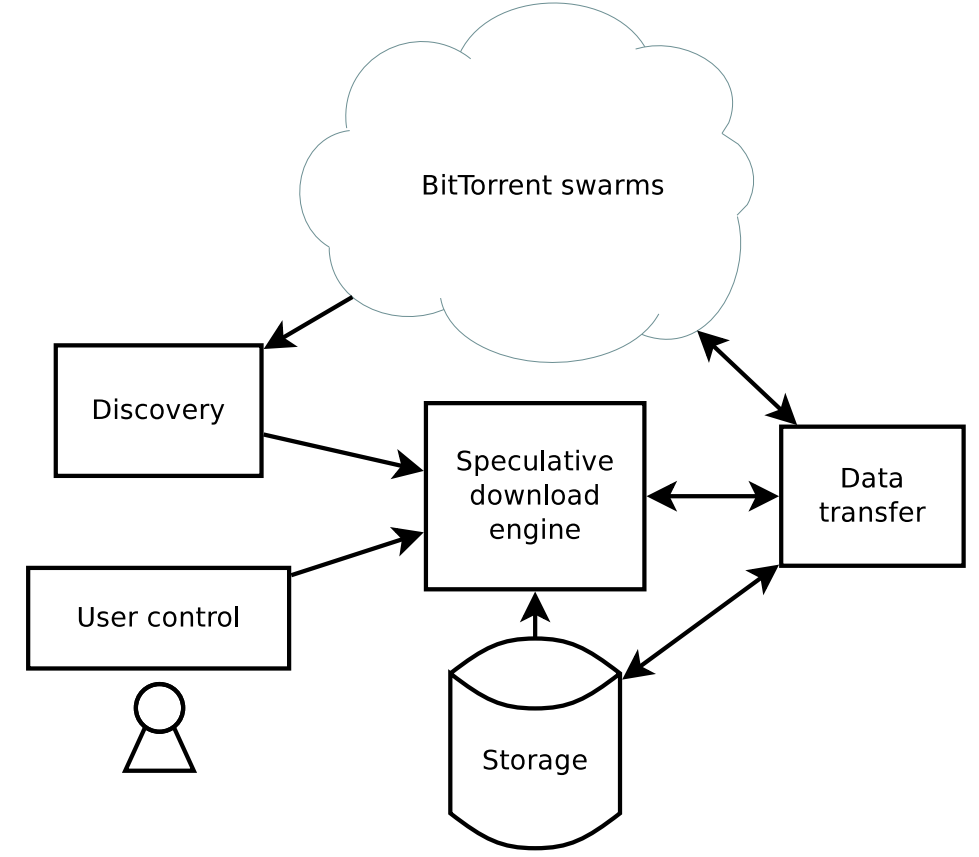
\includegraphics[width=0.7\textwidth]{pics/SDE2013.png}
	\caption{Speculative download mechanism \cite{2013:investmentcm:capota}}.
	\label{fig:sde13}
\end{figure}

In \citeyear{2013:investmentcm:capota}, \citeauthor{2013:investmentcm:capota} introduced bandwidth investing in \bt~private communities. He applied speculative download (as shown in figure \ref{fig:sde13}) on prospected swarm. This research used activity data crawled from Bitsoup\footnote{\url{https://www.bitsoup.me}} to evaluate their system. Every swarm is analyzed whether it will keep the swarm in \textit{cache} or discard it. Swarm is scored by predicting future upload speed defined in multiple regression model\cite{2013:investmentcm:capota}. One of the findings is that this algorithm depends on the size of the evaluated swarm. The more swarm need to be assessed, there is less chance the algorithm will find suitable cache to replace. This also shows the high costs and complexity of \textit{multivariate adaptive regression splines} (MARS) implemented in this system.

A year after, in \citeyear{2014:bwmarket:capota}, a research to align supply and demand in \bt~network is conducted. The idea is each peer monitor their swarms to detect whether there will be potential undersupply. If such a condition is found, one will broadcast \textit{help request} to specialized peers in order to seed this swarm. Specialized peers, called \textit{helpers}, tries to download as little as possible while upload as much as possible using \textit{libtorrent} share mode. They implement multiple helper and observe its effect to swarm with actual downloading on the other side. Their experiment result shows that using share mode in closed environment will increase download performance if the bandwidth is underutilized \cite{2014:bwmarket:capota} by shifting the bottleneck in the swarm. Moreover, \textit{libtorrent} share mode is also proven to be able to detect whether a swarm has enough capacity or not. This research also discussed flash crowd scenario. In this scenario, the existence of helper peer can lead leecher peer to reach higher download speed, especially in the early time of scenario. 

\begin{figure}[h]
	\centering
	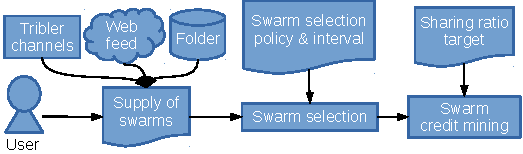
\includegraphics[width=0.8\textwidth]{pics/creditmining2015.pdf}
	\caption{The overview of credit mining process \cite{2015:creditmining:capota}}.
	\label{fig:cm15}
\end{figure}

The most recent work was conducted in \citeyear{2015:creditmining:capota}\cite{2015:creditmining:capota}. \citeauthor{2015:creditmining:capota} incorporated his previous work into Credit Mining System (CMS) implemented in Tribler. CMS able to monitor multiple swarm in one moment, and then decide which swarm this system will donate its bandwidth to. It uses simpler policy on choosing swarm compared to multivariate regression model in \cite{2013:investmentcm:capota}. As policy input, CMS uses torrent parameters such as seeder and leecher number obtained from tracker/DHT, creation date, length, and many others. The overview of mining process is shown in figure \ref{fig:cm15}. The experiment was conducted in live fashion on RSS \textit{etree.org}\footnote{\url{http://bt.etree.org/rss/bt\_etree\_org.rdf}} public community. They observed \textit{net upload gain} which defined as difference of uploaded bytes and downloaded bytes. Proposed policy and framework resulted in positive effect to the community.

Recent work on helping other user or increasing downloading performance using \bt~ has been done. \citeauthor{2014:cloudseed:leon} uses \bt~ protocol to increase user download speed and at the same time reduce datacenters load. They analyze which swarm or file to help using user bandwidth information and number of connected user\cite{2014:cloudseed:leon}. From another perspective, \citeauthor{2015:coalitionbt:zhang} introduced the \textit{coalition} between \bt~ peers. Coalition is a set of peers that cooperate each other in regards to \bt~policy to minimize download completion time. They also propose coalition-compatible choking strategy to replace the current \bt~one. This research lead to significant performance improvement within the coalition \cite{2015:coalitionbt:zhang}. Although not using \bt~protocol, in \citeyear{2009:p2phelp:he}, \citeauthor{2009:p2phelp:he} proved that helper peer also can improve the streaming capacity in P2P system\cite{2009:p2phelp:he}. \citeauthor{2016:gameauctionp2pstream:mostafavi} extend this work by introducing auction aspect for uploader to choose which user will receive the bandwidth he donate \cite{2016:gameauctionp2pstream:mostafavi}. \citeauthor{2016:gameauctionp2pstream:mostafavi} used game-theory to propose new framework in uncooperative peers with maximizing the credit gain for helpers.



\section{P2P Currency}
% Some research has been conducted to tackle performance degradation in a swarm.
% some to increase throughput
Current currency used in Tribler (Multichain)\cite{2015:multichain:norberhuis}.\\ Demand and supply in bittorrent environment \cite{2009:demandsupplyres:andrade}.
Tracking back, generally, the core of credit mining try to solve supply and demand misalignment. \citeauthor{2011:interswarm:capota} in \citeyear{2011:interswarm:capota} showed that in private community \cite{2011:interswarm:capota}.